\section{\faWrench\ Docker Model Runner} % (fold)
\label{sec:spring-ai-project-setup}
%
\begin{frame}[t,fragile] \frametitle{Docker Model Runner}
    \framesubtitle{Descrizione}
    \begin{itemize}[leftmargin=10pt,align=right]
        \onslide<1->\item[\alert{\faArrowCircleRight}] Risposta di Docker ad Ollama
        \onslide<2->
        \begin{itemize}[leftmargin=10pt,align=right]
            \item[\alert{\faArrowCircleRight}] LLM in Docker \textit{container} locali
            \item[\alert{\faArrowCircleRight}] Modelli AI generici dockerizzabili (WIP)
            \item[\alert{\faArrowCircleRight}] Docker mette a disposizione una serie di modelli \textit{open source} scaricabili tramite Engine o Desktop
        \end{itemize}

        \onslide<3->\item[\alert{\faArrowCircleRight}] Requisiti: {\footnotesize \url{https://www.ajeetraina.com/docker-model-runner-tutorial-and-cheatsheet-mac-windows-and-linux-support/}}

    \onslide<4->\item[\alert{\faExternalLink}] {\footnotesize \url{https://docs.docker.com/ai/model-runner/}}
    \item[\alert{\faExternalLink}] {\footnotesize \url{https://www.docker.com/blog/run-llms-locally/}}
    \item[\alert{\faExternalLink}] {\footnotesize \url{https://www.docker.com/blog/introducing-docker-model-runner/}}
    \end{itemize}
\end{frame}
%
\begin{frame}[t,fragile] \frametitle{Docker Model Runner}
    \framesubtitle{Come si usa?}
    \begin{itemize}[leftmargin=10pt,align=right]
        \onslide<1->\item[\alert{\faArrowCircleRight}] Tramite Docker Engine
        \onslide<2->\item[\alert{\faArrowCircleRight}] Tramite Docker Desktop
    \end{itemize}
\end{frame}
%
\begin{frame}[t,fragile] \frametitle{Docker Model Runner}
    \framesubtitle{Utilizzo di base - Docker Engine}
        \begin{codeblock}{Caricamento LLM in locale}
            \begin{minted}{shell-session}
            docker model pull ai/gemma3
            \end{minted}
        \end{codeblock}
        \begin{codeblock}{Esecuzione LLM in locale}
            \begin{minted}{shell-session}
            docker model run ai/gemma3
            \end{minted}
        \end{codeblock}
        \begin{codeblock}{Elenco LLM in locale}
            \begin{minted}{shell-session}
            docker model list
            \end{minted}
        \end{codeblock}
        \begin{codeblock}{Eliminazione LLM in locale}
            \begin{minted}{shell-session}
            docker model rm ai/gemma3
            \end{minted}
        \end{codeblock}
\end{frame}
%
\begin{frame}[t,fragile] \frametitle{Docker Model Runner}
\framesubtitle{Utilizzo di base - Docker Desktop}
	\vspace*{-.5cm}
    {\footnotesize
    \begin{itemize}
        \only<1|handout:1>{\item[\alertedcircled{1}] Verificare le impostazioni relative ad \texttt{AI}}
        \only<2|handout:2>{\item[\alertedcircled{2}] Verificare le impostazioni relative alle \texttt{Beta features}}
        \only<3|handout:3>{\item[\alertedcircled{3}] Accedere al pannello \texttt{Docker Hub} della sezione \texttt{Models}}
        \only<4|handout:4>{\item[\alertedcircled{4}] Selezionare il modello ed eventuale versionamento quantizzato}
        \only<5|handout:5>{\item[\alertedcircled{5}] Utilizzare il modello da linea di comando integrata}
    \end{itemize}
    }
    \vfill
    \begin{minipage}[b]{\textwidth}
		\centering
        \only<1|handout:1>{
		    \begin{figure}[ht]
			    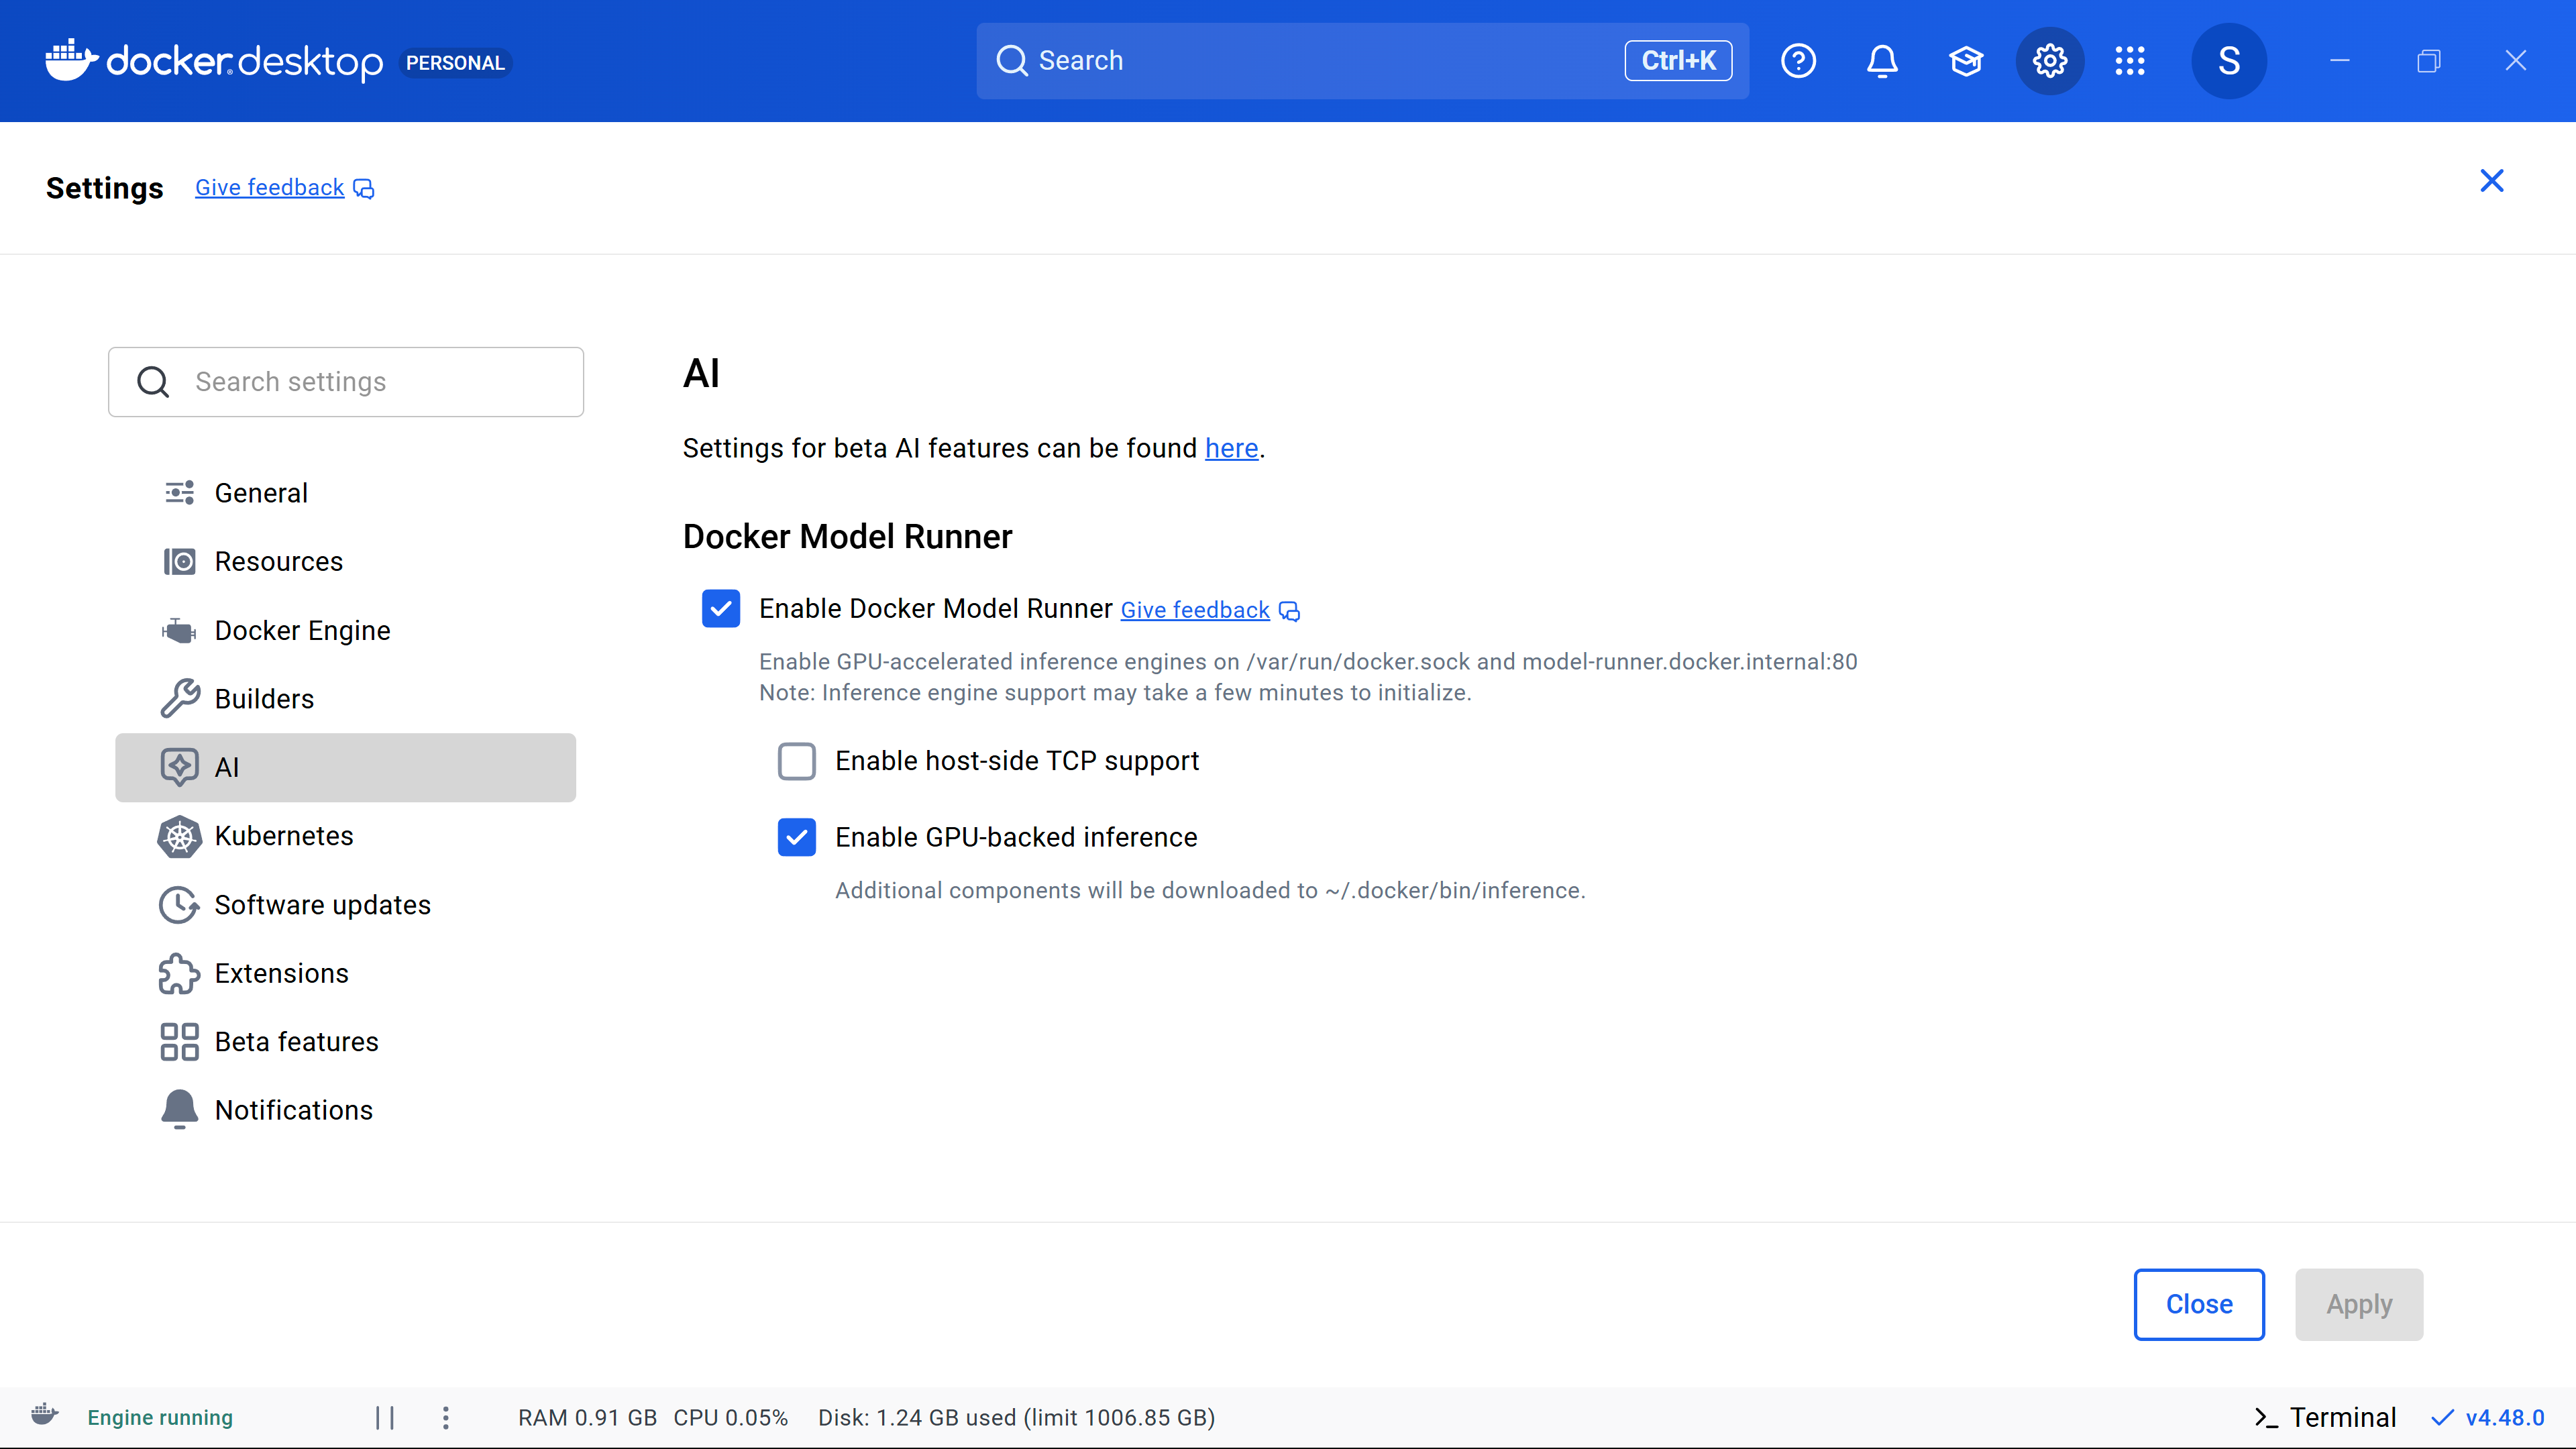
\includegraphics[width=\textwidth, frame]{img/docker-desktop-model-runner-ai.png}
		    \end{figure}
        }
         \only<2|handout:2>{
		    \begin{figure}[ht]
			    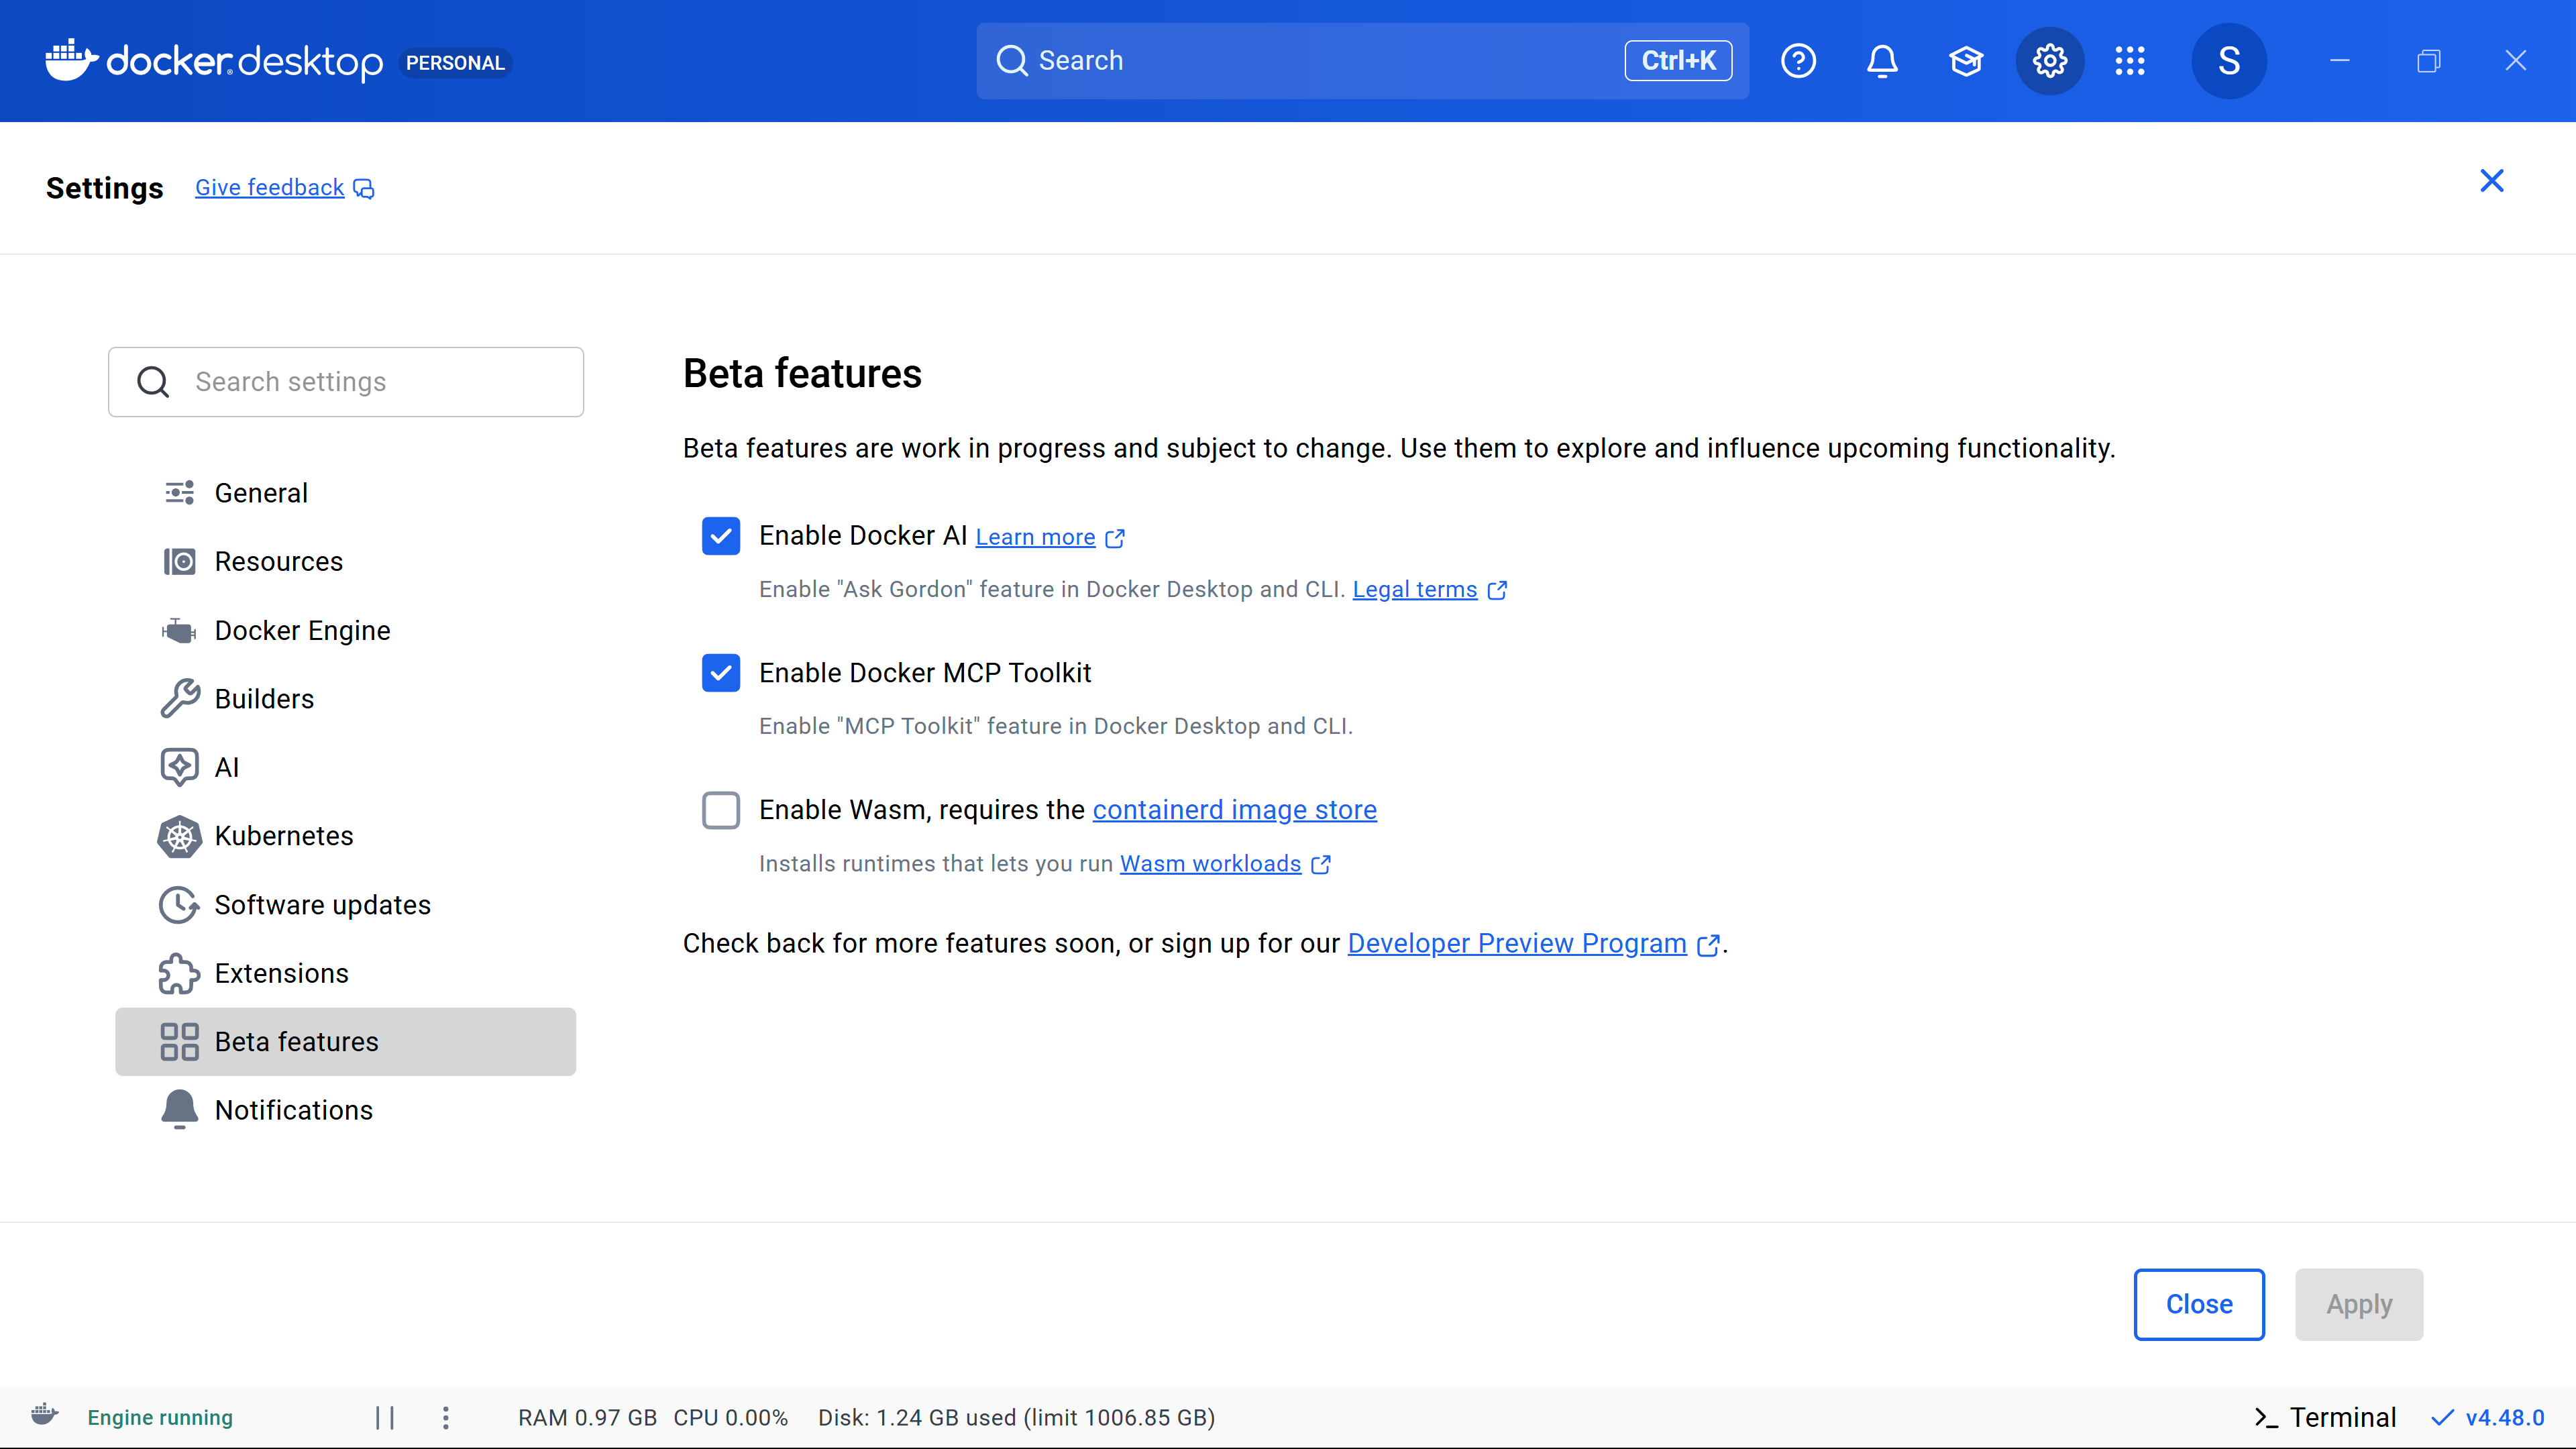
\includegraphics[width=\textwidth, frame]{img/docker-desktop-model-runner-beta-features.png}
		    \end{figure}
        }
        \only<3|handout:3>{
		    \begin{figure}[ht]
			    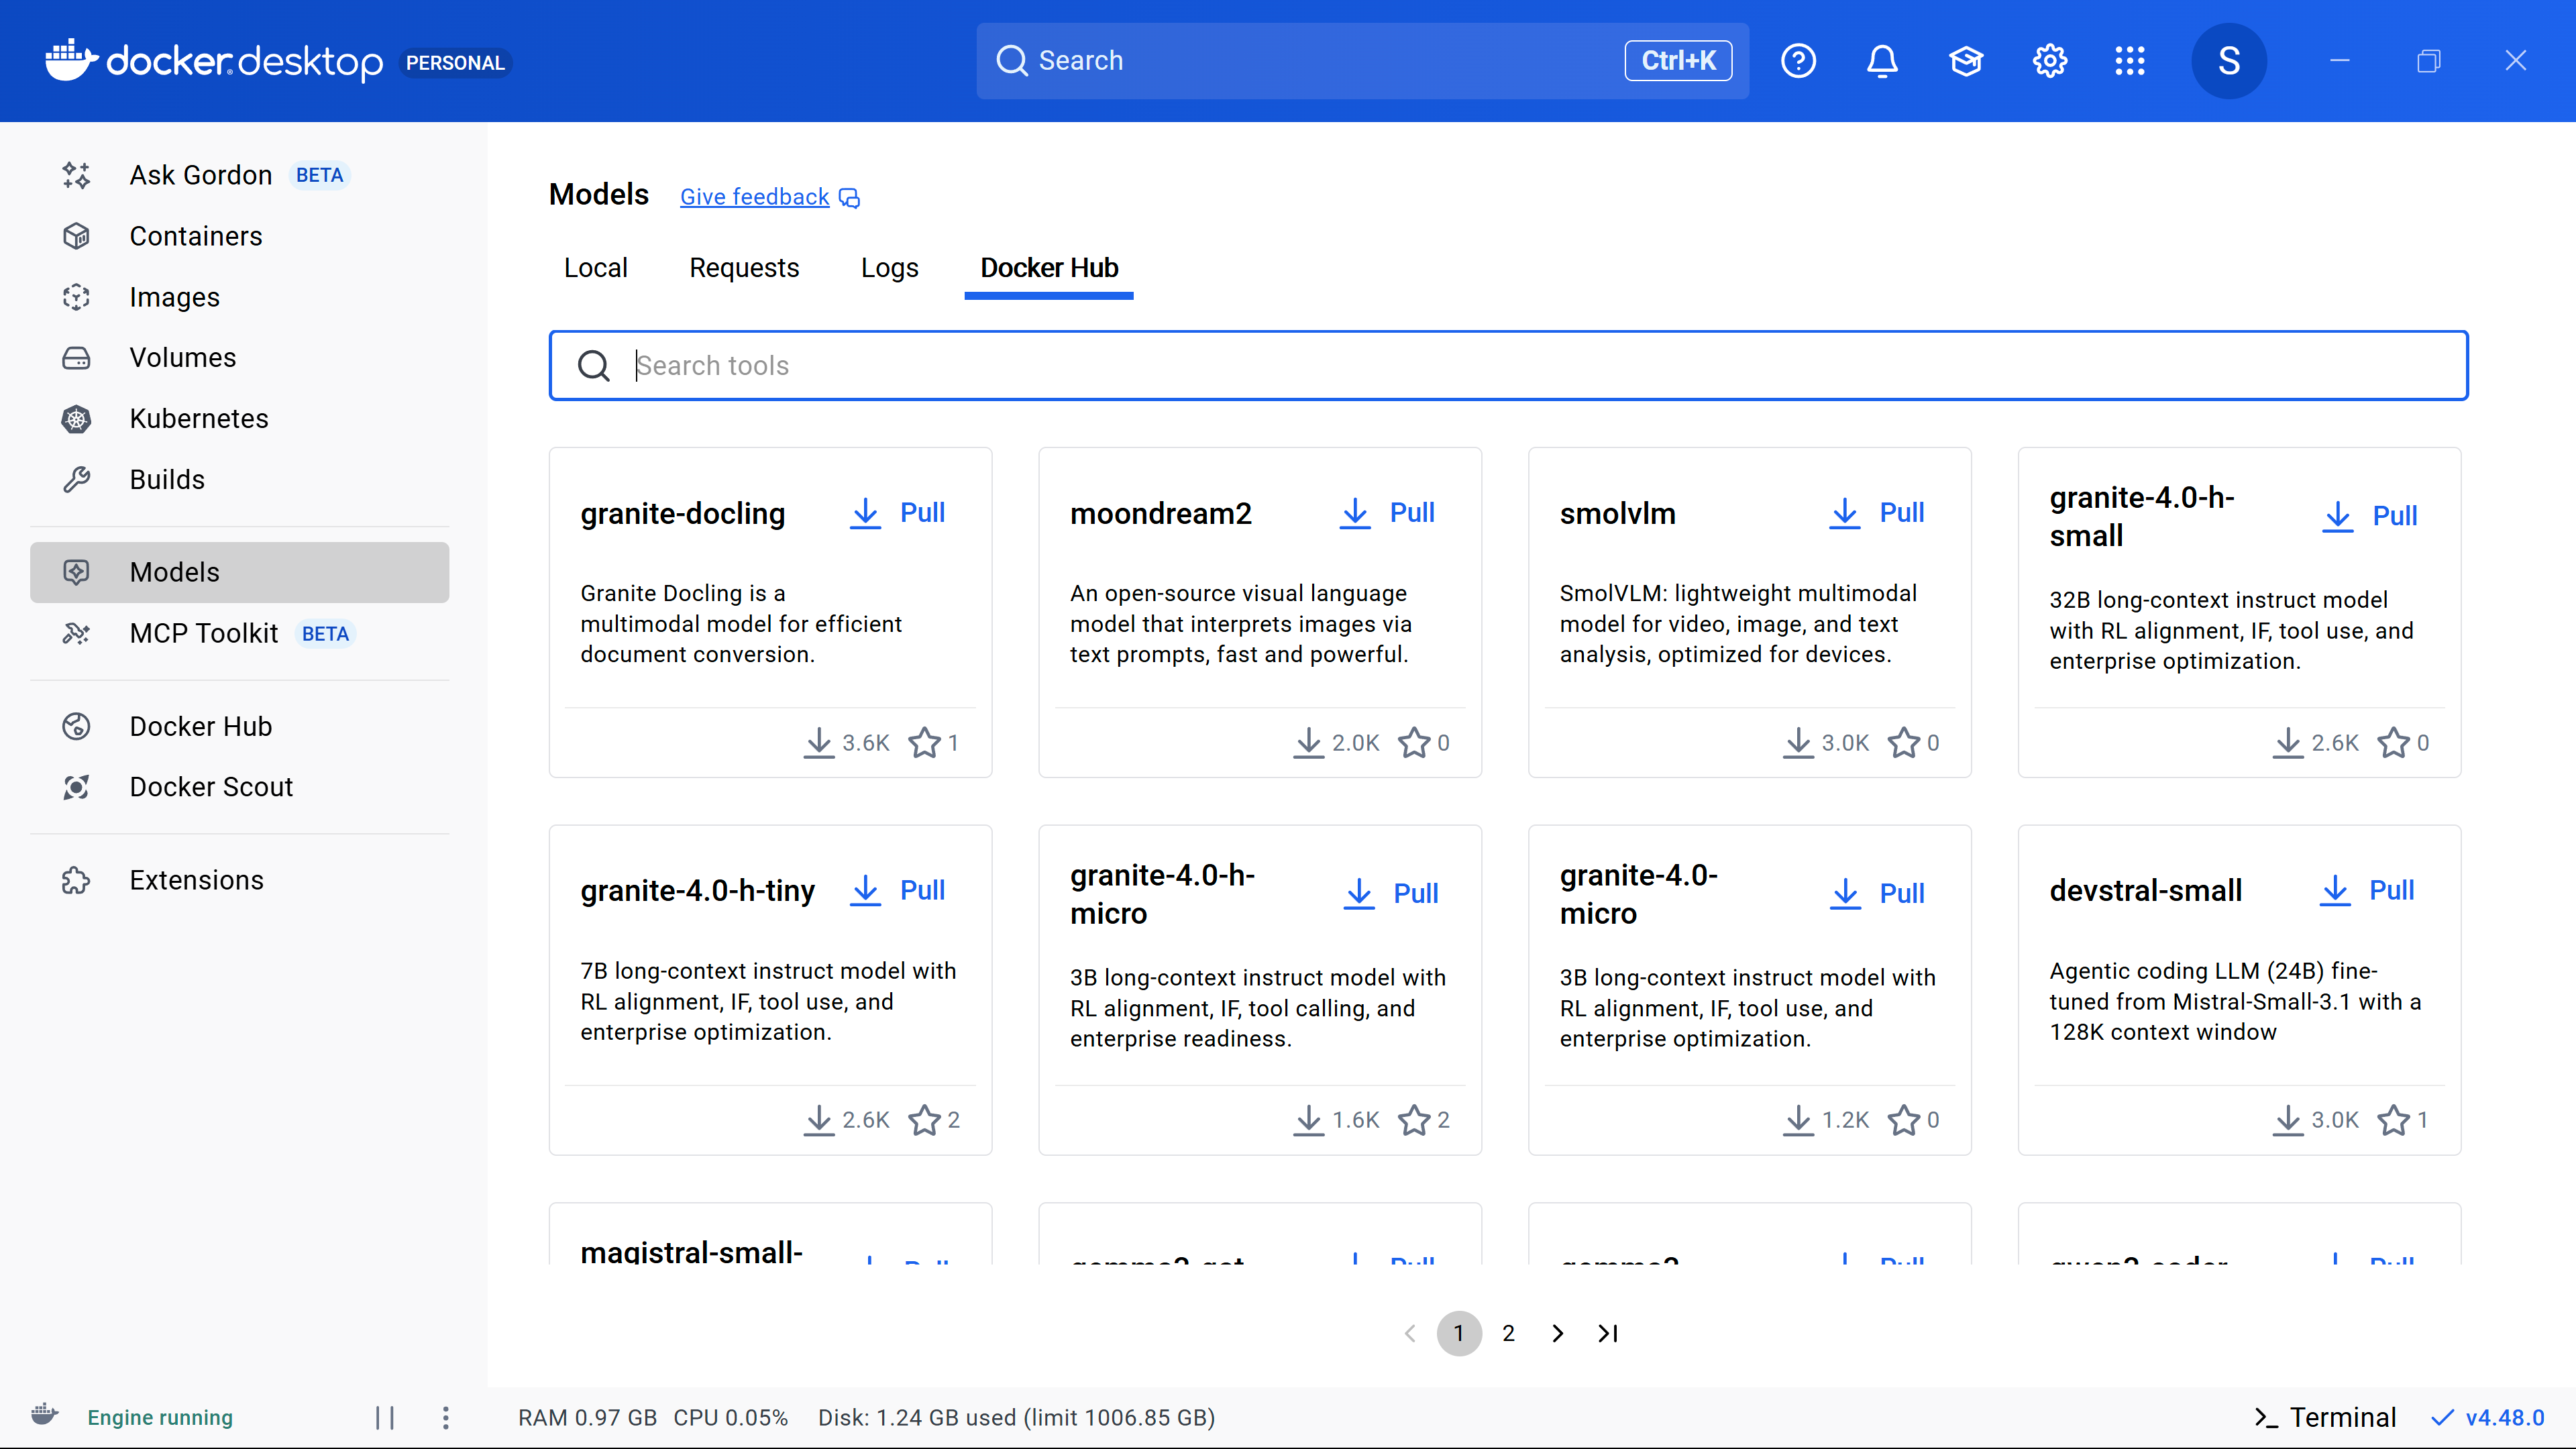
\includegraphics[width=\textwidth, frame]{img/docker-desktop-model-runner-hub.png}
		    \end{figure}
        }
        \only<4|handout:4>{
		    \begin{figure}[ht]
			    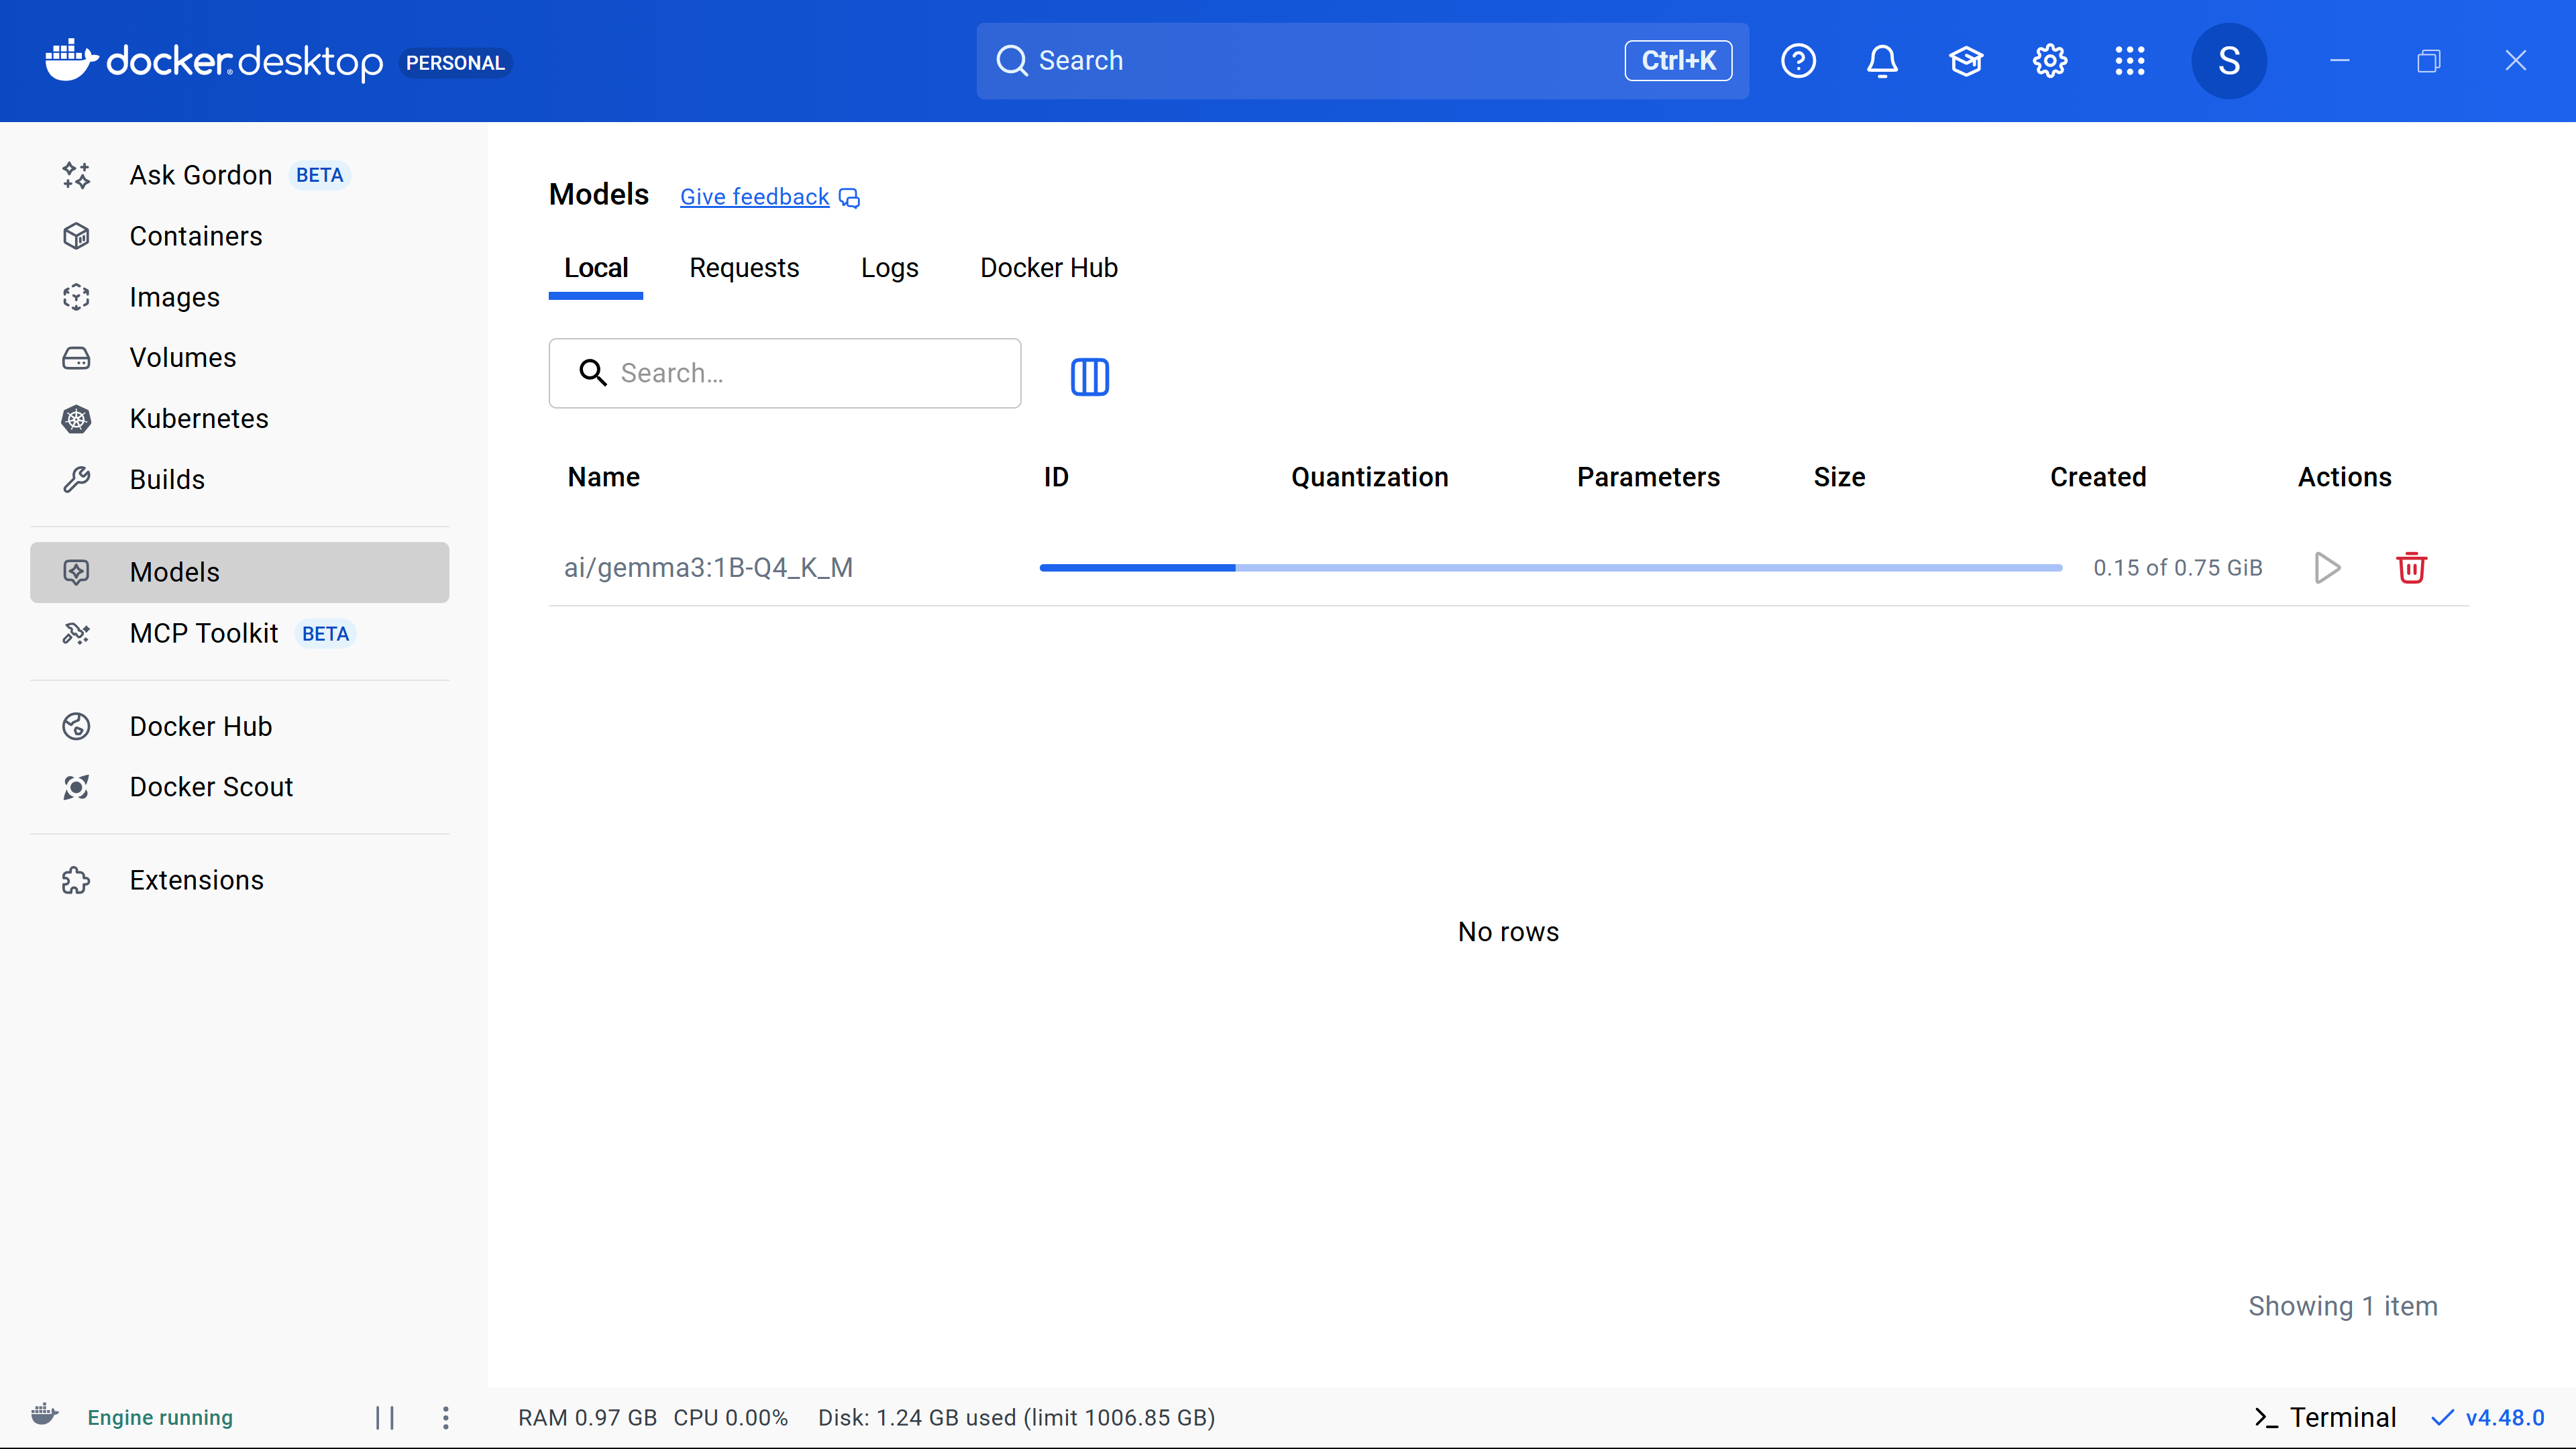
\includegraphics[width=\textwidth, frame]{img/docker-desktop-model-runner-download.png}
		    \end{figure}
        }
        \only<5|handout:5>{
		    \begin{figure}[ht]
			    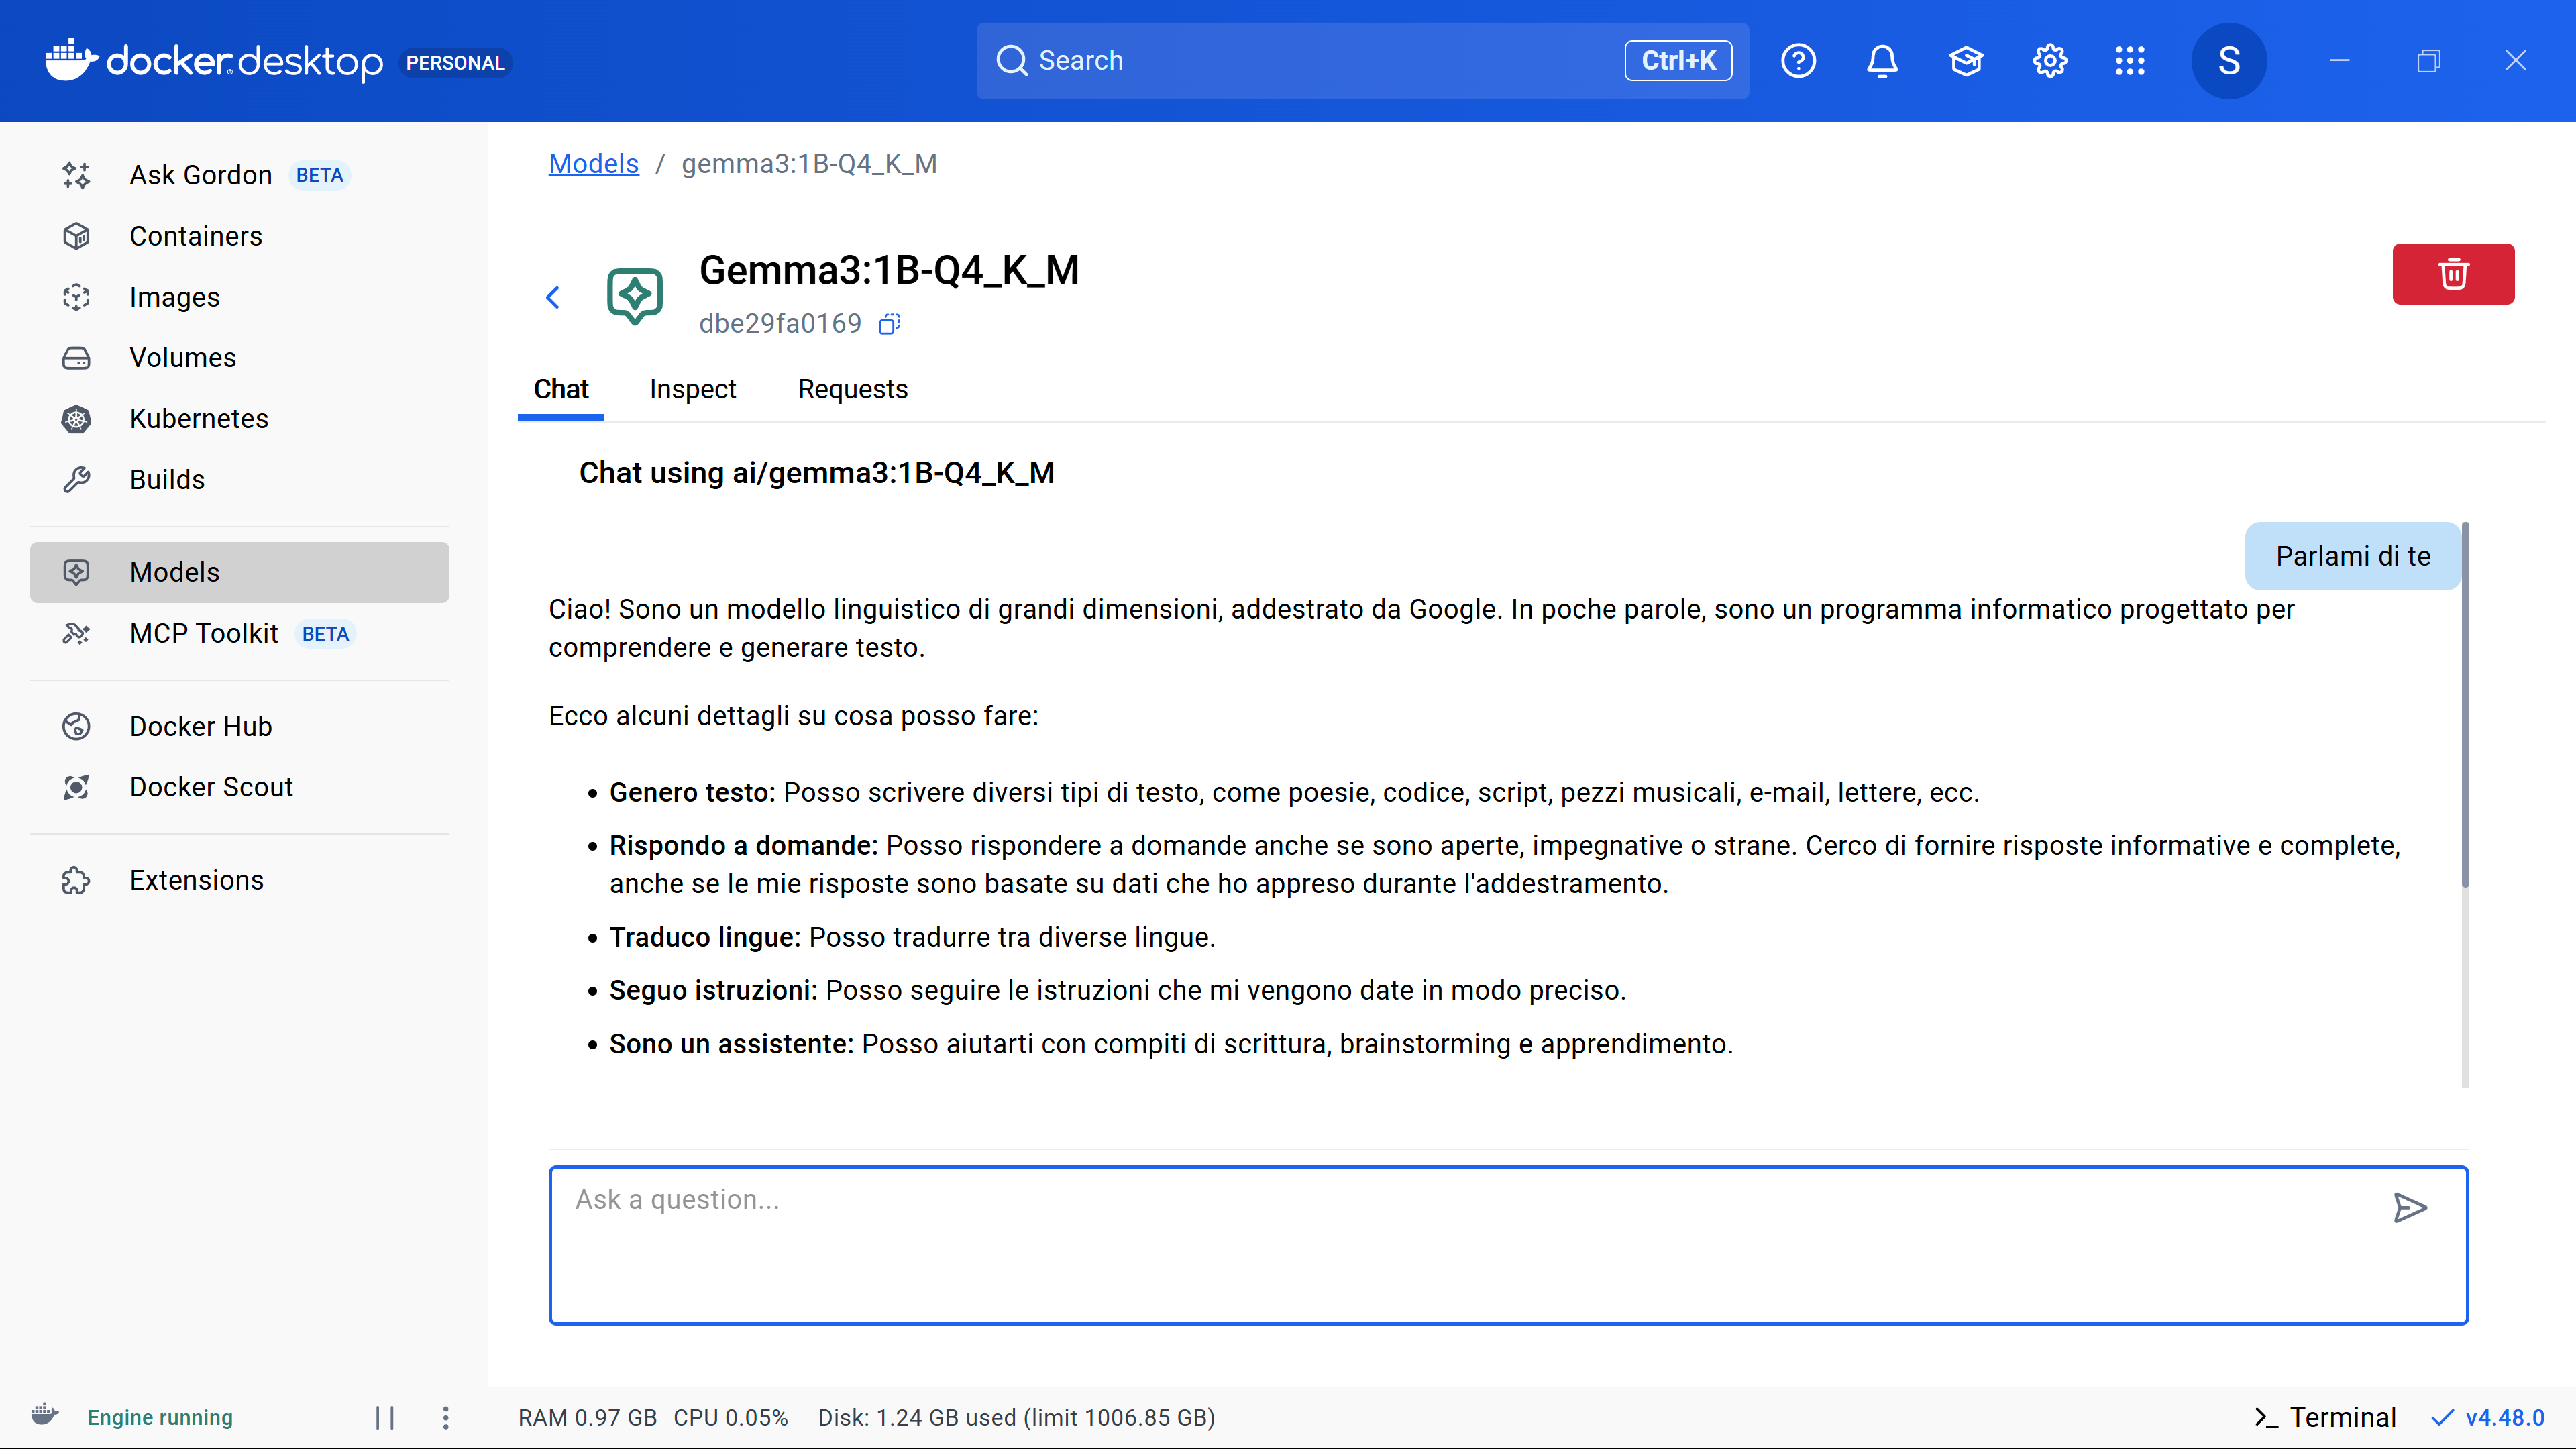
\includegraphics[width=\textwidth, frame]{img/docker-desktop-model-runner-model-inference.png}
		    \end{figure}
        }
	\end{minipage}
\end{frame}
%
\begin{frame}[t,fragile] \frametitle{Docker Model Runner}
    \framesubtitle{Integrazione in Spring AI}
    \begin{itemize}[leftmargin=10pt,align=right]
        \onslide<1->\item[\alert{\faArrowCircleRight}] Come fosse un servizio \alert{OpenAI}!
    \end{itemize}
        \onslide<2->
        \begin{block}{\textit{File} \texttt{pom.xml}}
			{\tiny\inputminted{xml}{code/pom.xml}}
    	\end{block}
        \onslide<3->
        \begin{block}{\textit{File} \texttt{application.yml}}
			{\tiny\inputminted{yaml}{code/application.yml}}
    	\end{block}
\end{frame}